\documentclass[12pt]{article}
\usepackage[a4paper, margin=1in]{geometry}
\usepackage{graphicx}
\usepackage{amsmath}
\usepackage{float}
\usepackage{hyperref}
\usepackage{caption}
\usepackage{subcaption}
\usepackage{color}

\title{\textbf{Image Stitching}}
\author{Niladri Ghosh \\
ID-B2430100 \\
Department of Computer Science}
\date{\today}

\begin{document}

\maketitle

\begin{abstract}
This report presents an advanced implementation of image stitching using SIFT (Scale-Invariant Feature Transform) for keypoint detection and description, followed by feature matching and homography estimation using RANSAC. A key enhancement in this project is the inclusion of a smoothing mask to apply multi-band blending for seamless transition across the overlapping regions of images. The result is a more coherent and natural panoramic image.
\end{abstract}

\section{Introduction}
Image stitching is a key task in computer vision that involves combining two or more images to create a panorama. Traditional stitching pipelines face issues like visible seams and lighting mismatches. To mitigate these, this project uses:
\begin{itemize}
    \item \textbf{SIFT} for scale- and rotation-invariant feature detection.
    \item \textbf{Ratio test} for filtering reliable matches.
    \item \textbf{RANSAC} for robust homography estimation.
    \item \textbf{Multi-band blending masks} for smooth merging of overlapping areas.
\end{itemize}

\section{Methodology}

\subsection{Feature Detection and Matching}
Features are detected using SIFT, and matches are filtered using Lowe’s ratio test to retain reliable correspondences.

\begin{verbatim}
self.sift = cv2.SIFT_create()
kp1, des1 = self.sift.detectAndCompute(img1, None)
kp2, des2 = self.sift.detectAndCompute(img2, None)
\end{verbatim}

The best matches are drawn and saved using OpenCV for visualization. An example is shown in Figure \ref{fig:matches}.

\begin{figure}[H]
    \centering
    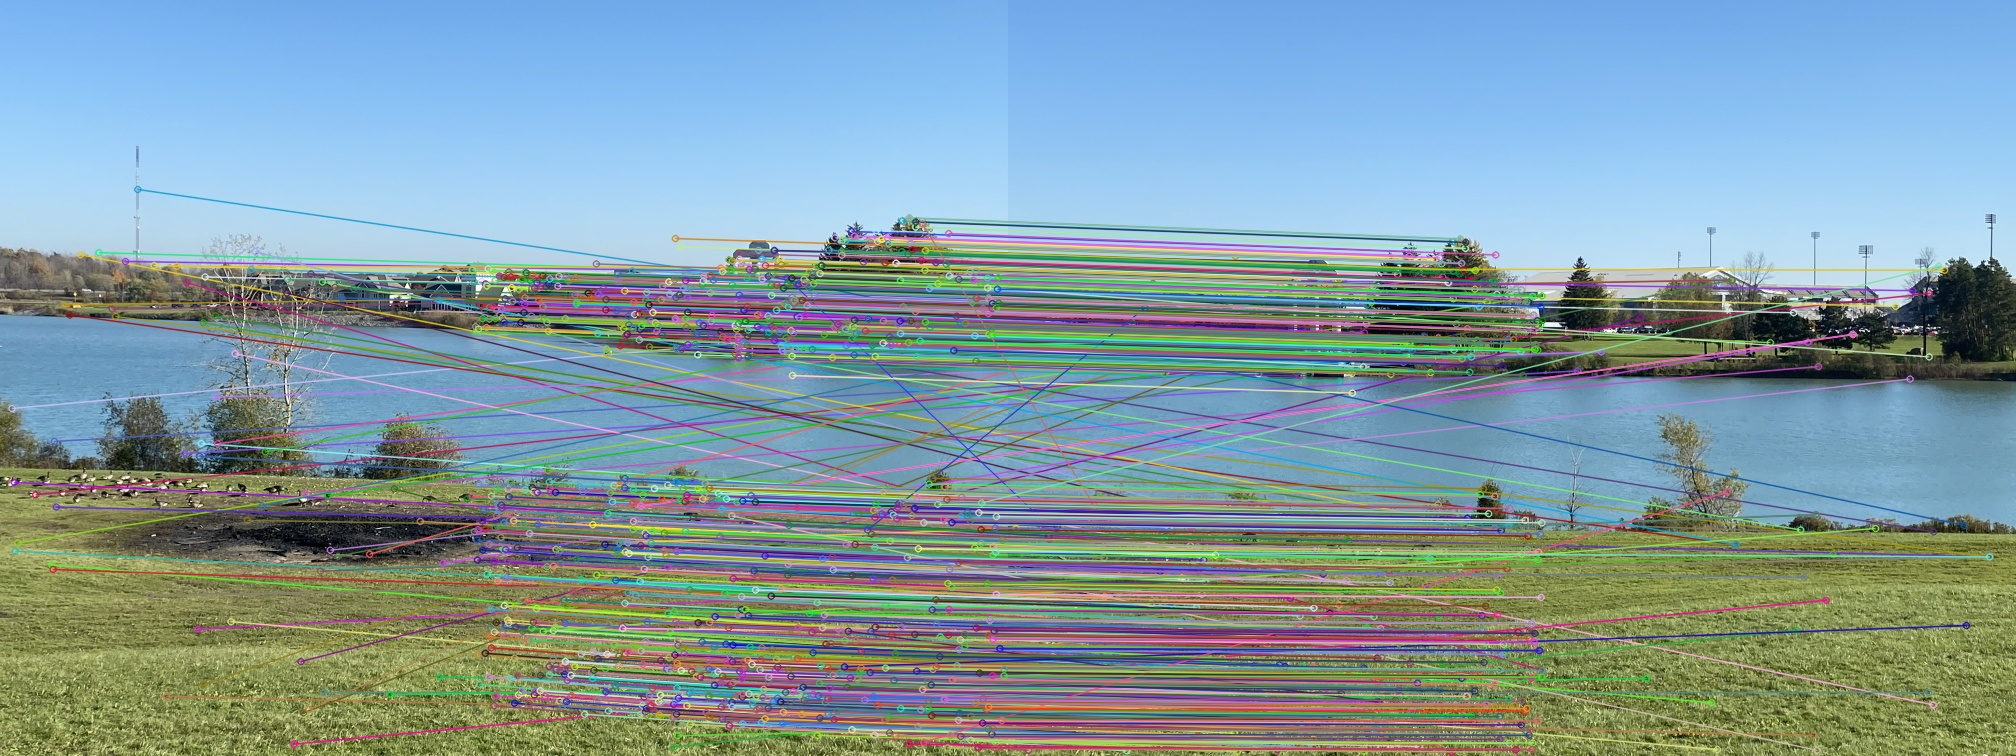
\includegraphics[width=0.8\textwidth]{matching1.jpg}
    \caption{Feature Matches between Images}
    \label{fig:matches}
\end{figure}

\subsection{Homography Estimation}
Using the good matches, a homography matrix is calculated using the RANSAC algorithm, which helps to reject outliers and accurately align the images.

\begin{verbatim}
H, status = cv2.findHomography(image2_kp, image1_kp, cv2.RANSAC, 5.0)
\end{verbatim}

\subsection{Blending with Smoothing Masks}
To blend images seamlessly, two masks are created:
\begin{itemize}
    \item A left-image mask that gradually decreases from left to right.
    \item A right-image mask that increases from left to right.
\end{itemize}

These masks allow overlapping regions to be combined smoothly without harsh transitions.

\begin{figure}[H]
    \centering
    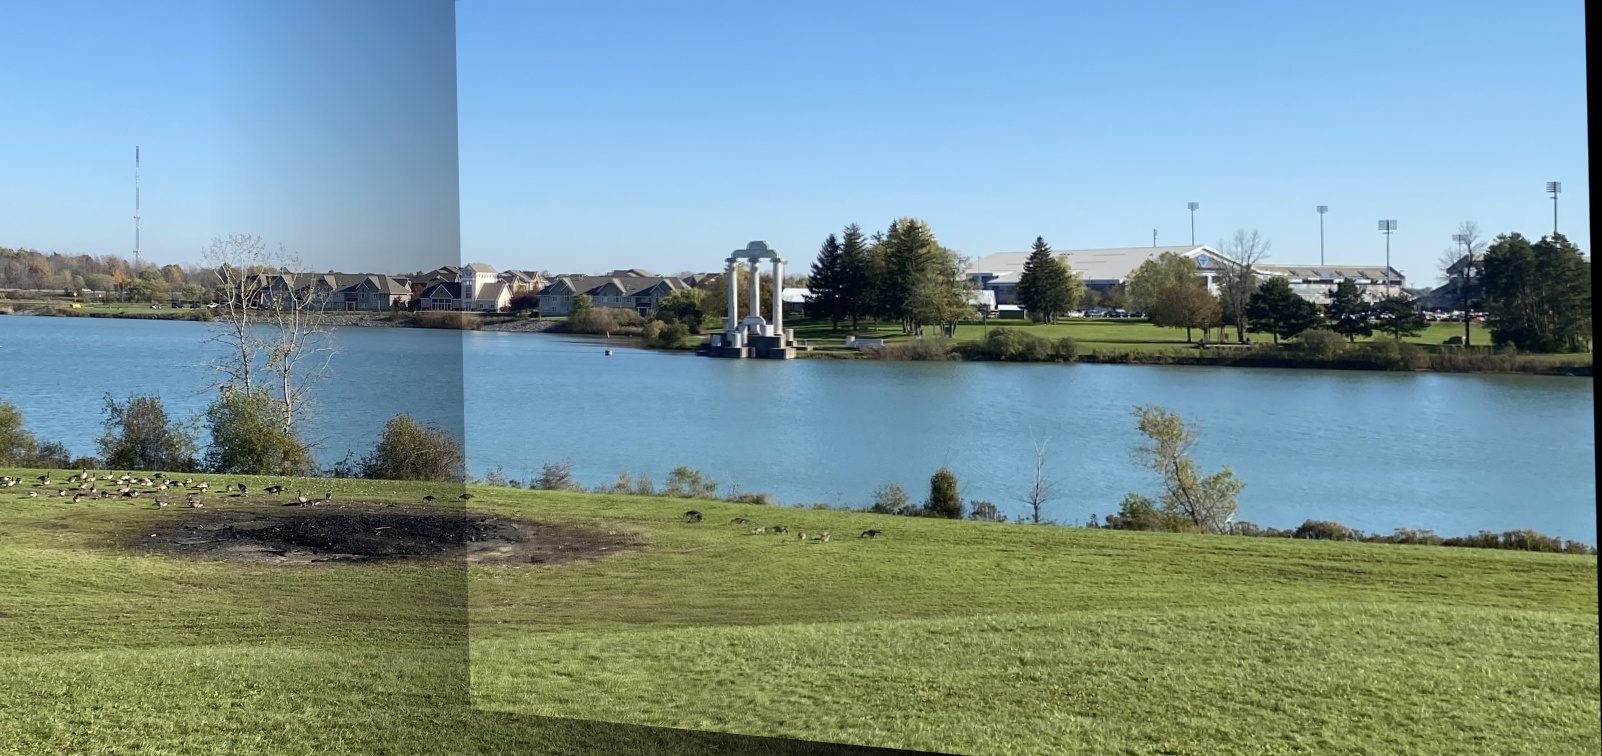
\includegraphics[width=0.95\textwidth]{panorama 1.jpg}
    \caption{Final Stitched Panorama (First Pair)}
\end{figure}

\subsection{Warping and Cropping}
The second image is warped using the homography matrix and then added to the base canvas with the left image. Post-blending, the image is cropped to remove any black borders.

\begin{verbatim}
rows, cols = np.where(result[:, :, 0] != 0)
final_result = result[min_row:max_row, min_col:max_col, :]
\end{verbatim}

\begin{figure}[H]
    \centering
    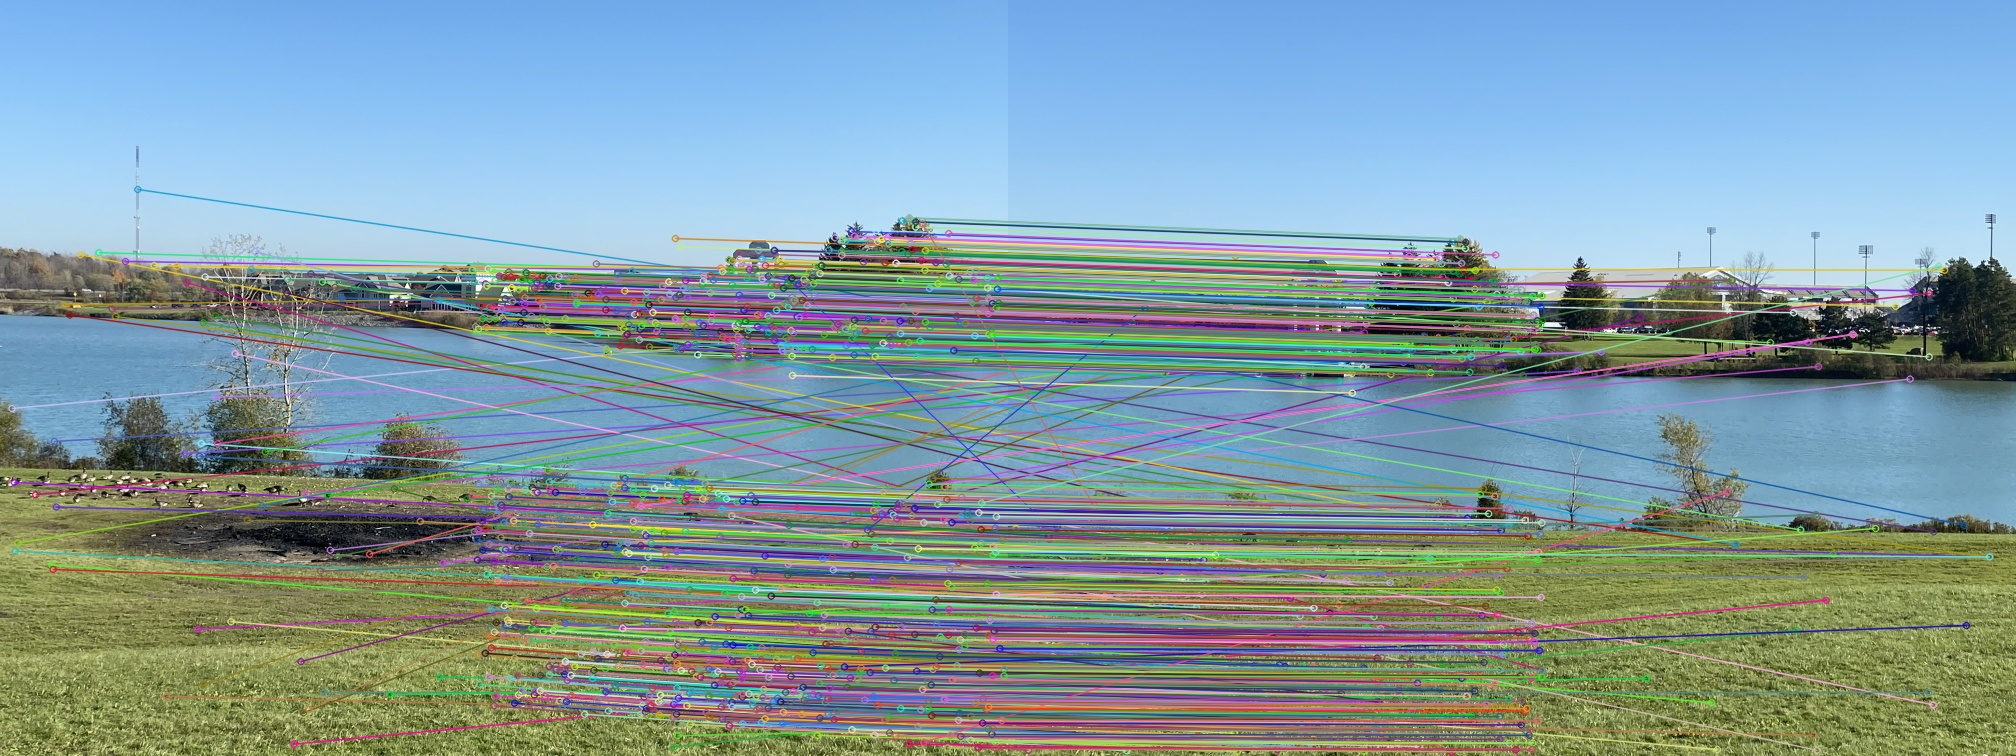
\includegraphics[width=0.95\textwidth]{matching1.jpg}
    \caption{Final Stitched Panorama (Second Pair)}
\end{figure}

\section{Results} 
I have used my images to implement this practically.
\begin{figure}[H]
    \centering
    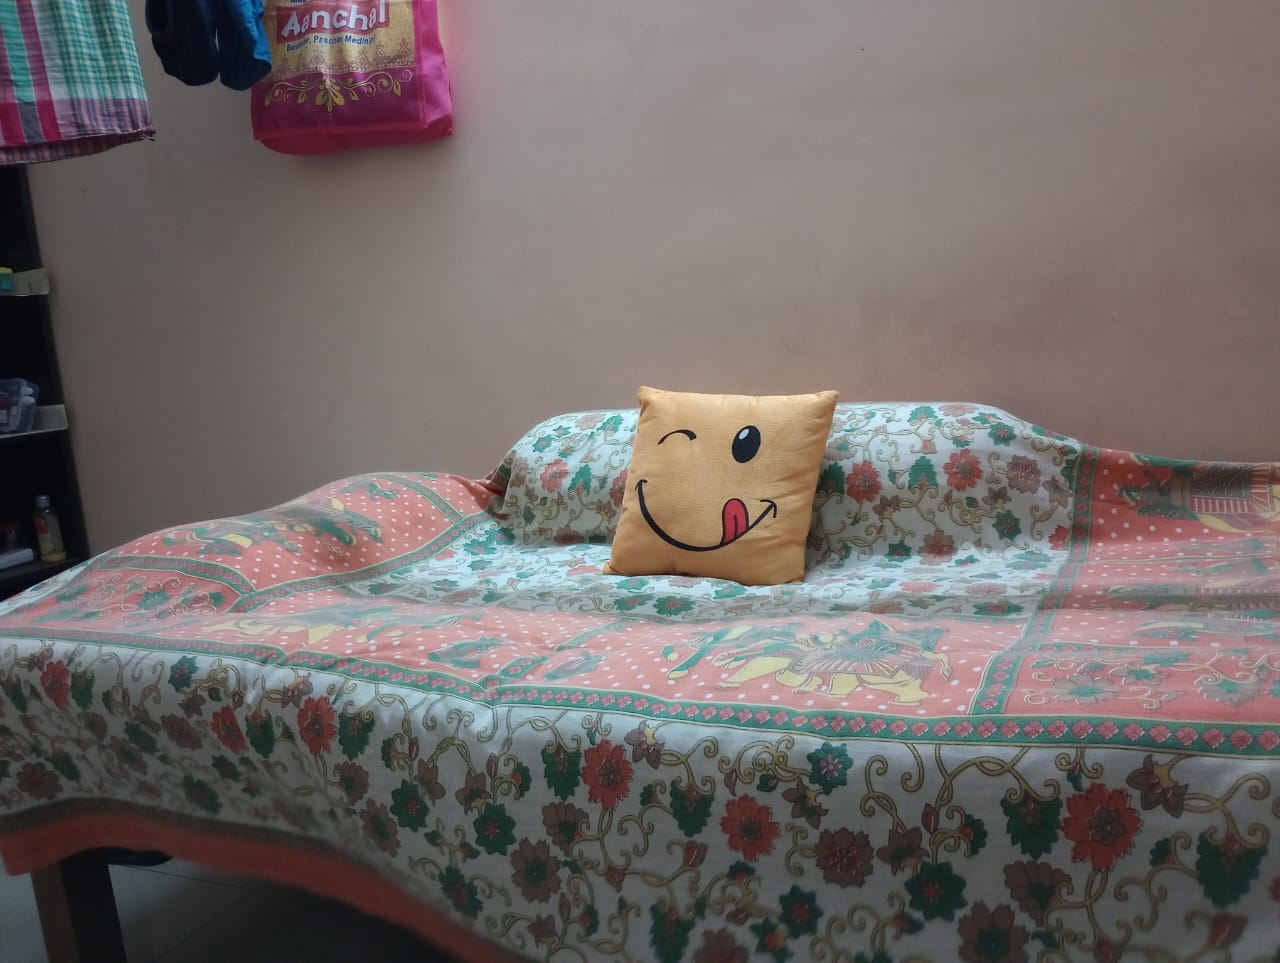
\includegraphics[width=0.8\textwidth]{left2.jpg}
    \caption{left image}
    \label{fig:matches}
\end{figure}
\begin{figure}[H]
    \centering
    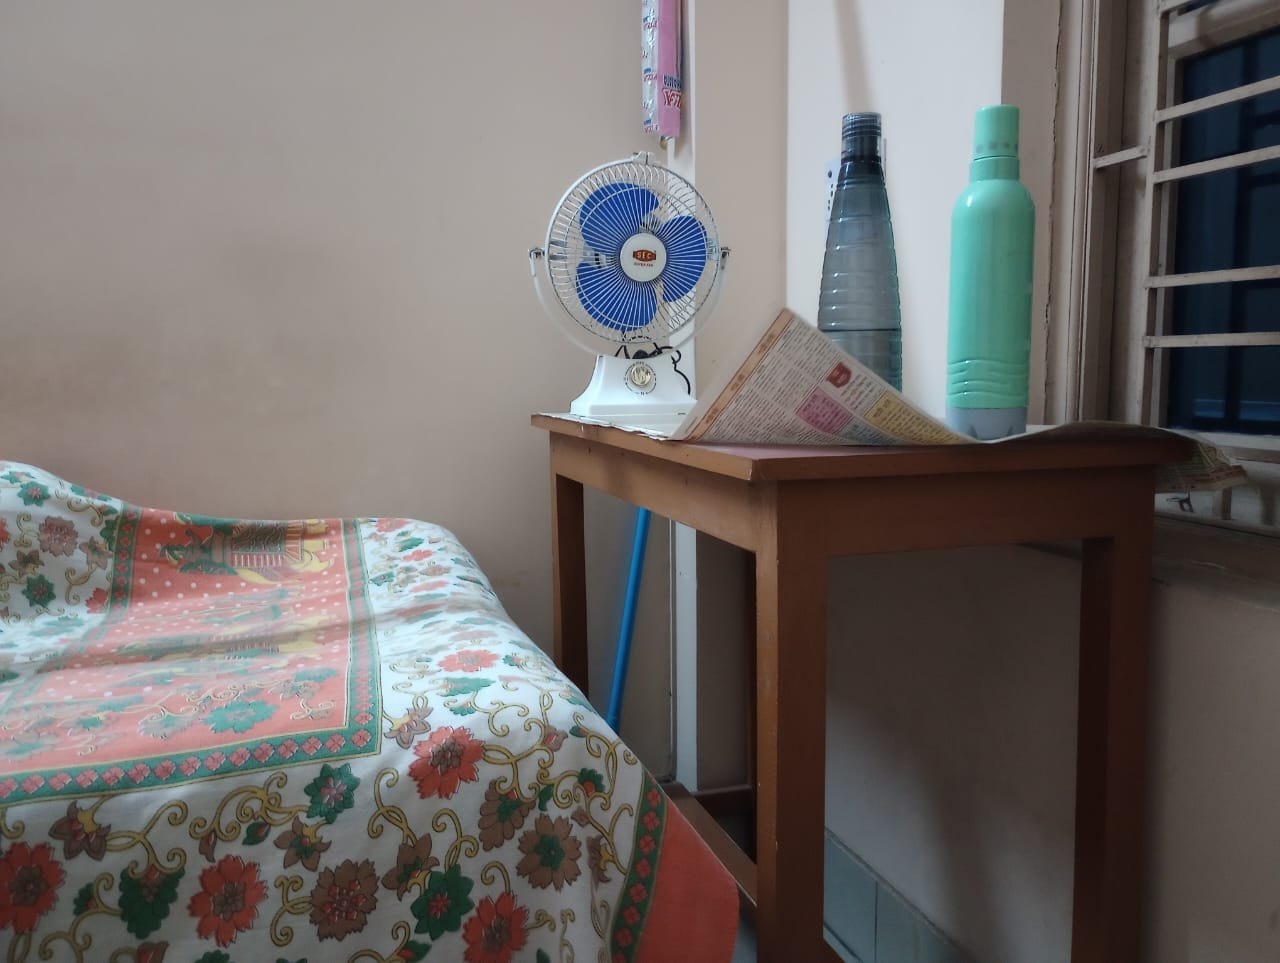
\includegraphics[width=0.8\textwidth]{right2.jpg}
    \caption{right image}
    \label{fig:matches}
\end{figure}
\begin{figure}[H]
    \centering
    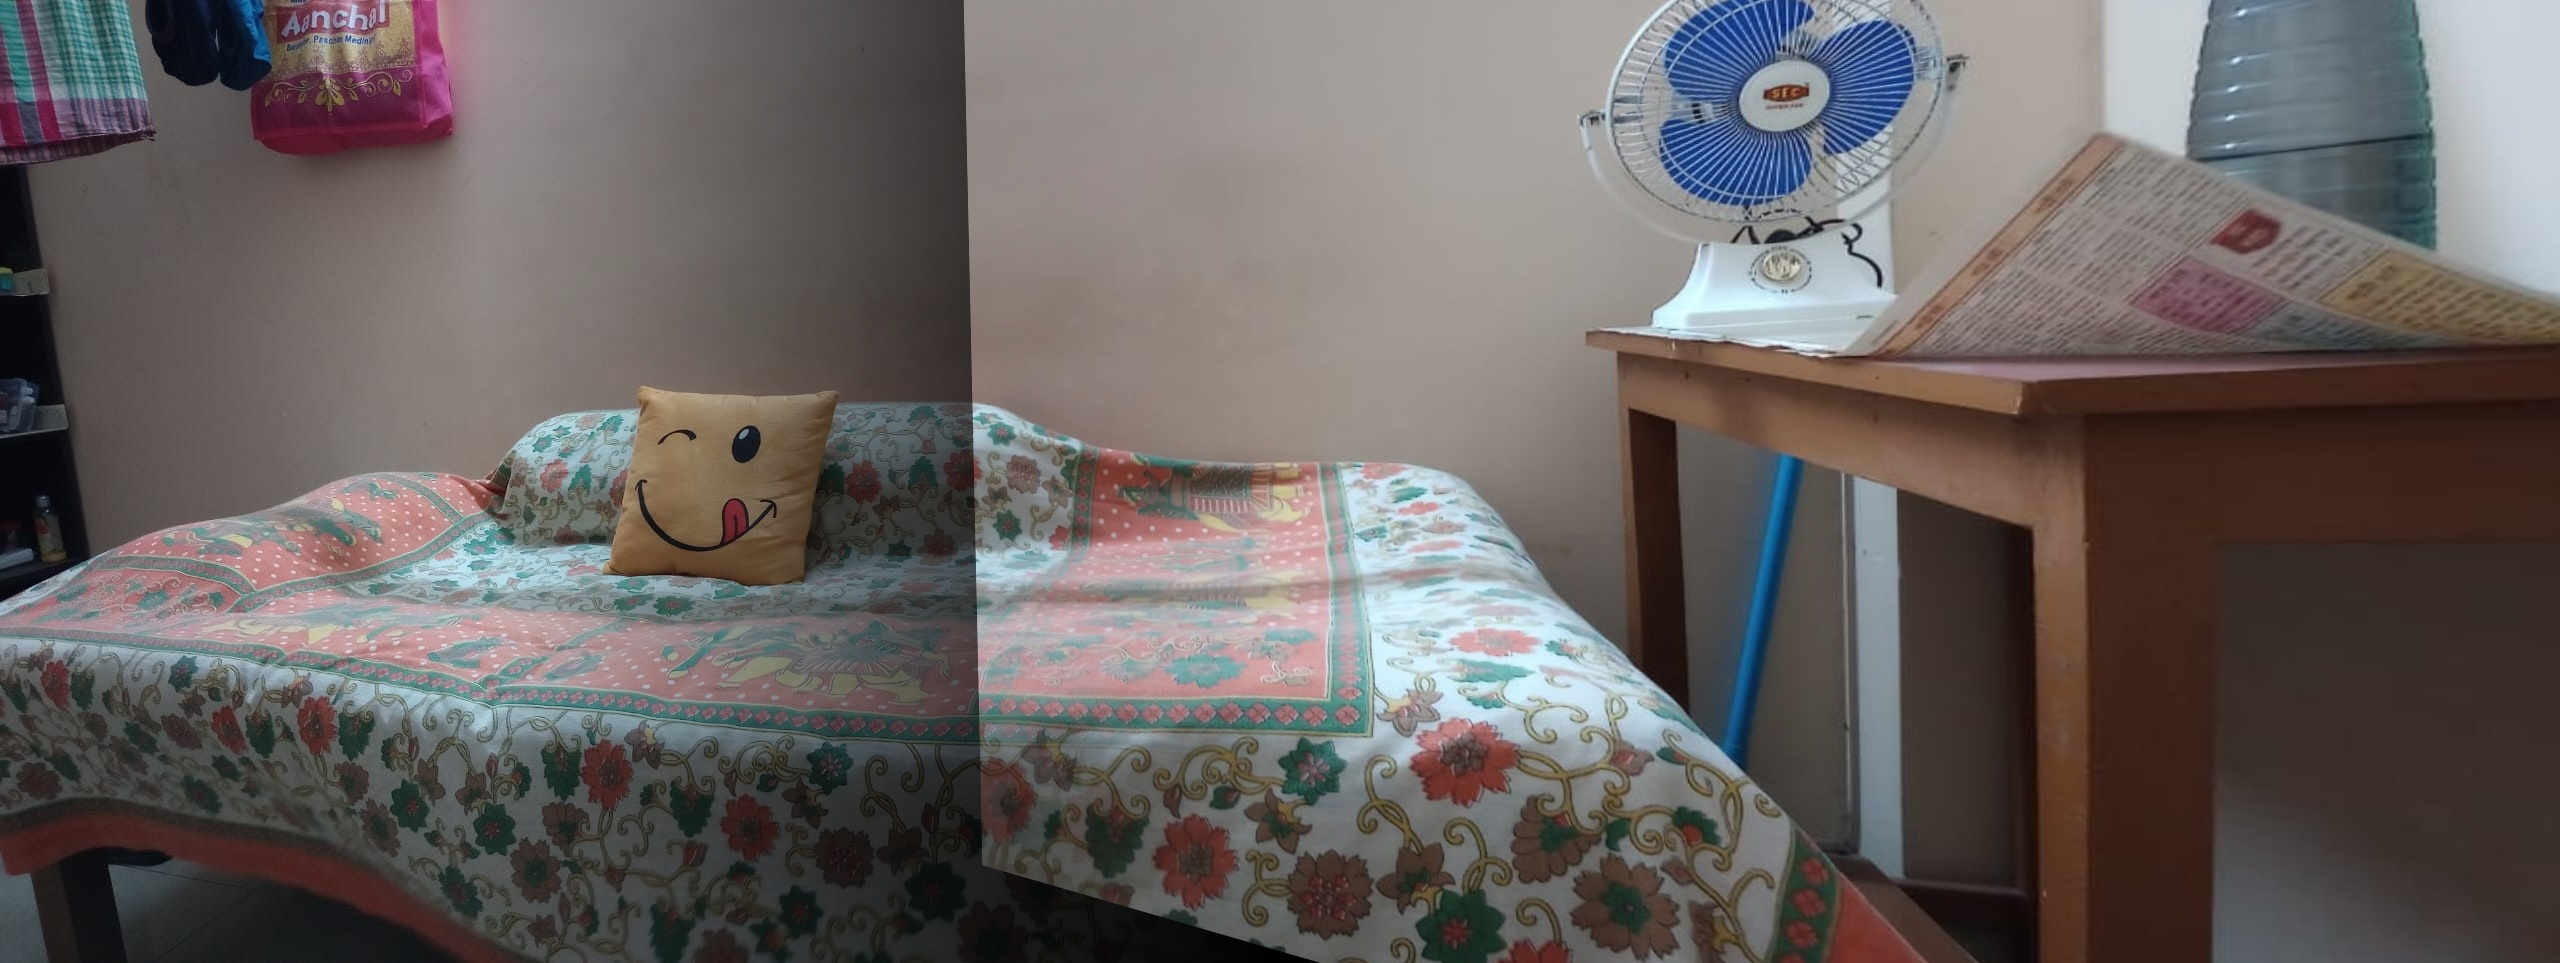
\includegraphics[width=0.8\textwidth]{panorama 2.jpg}
    \caption{Image Stiching}
    \label{fig:matches}
\end{figure}
\begin{figure}[H]
    \centering
    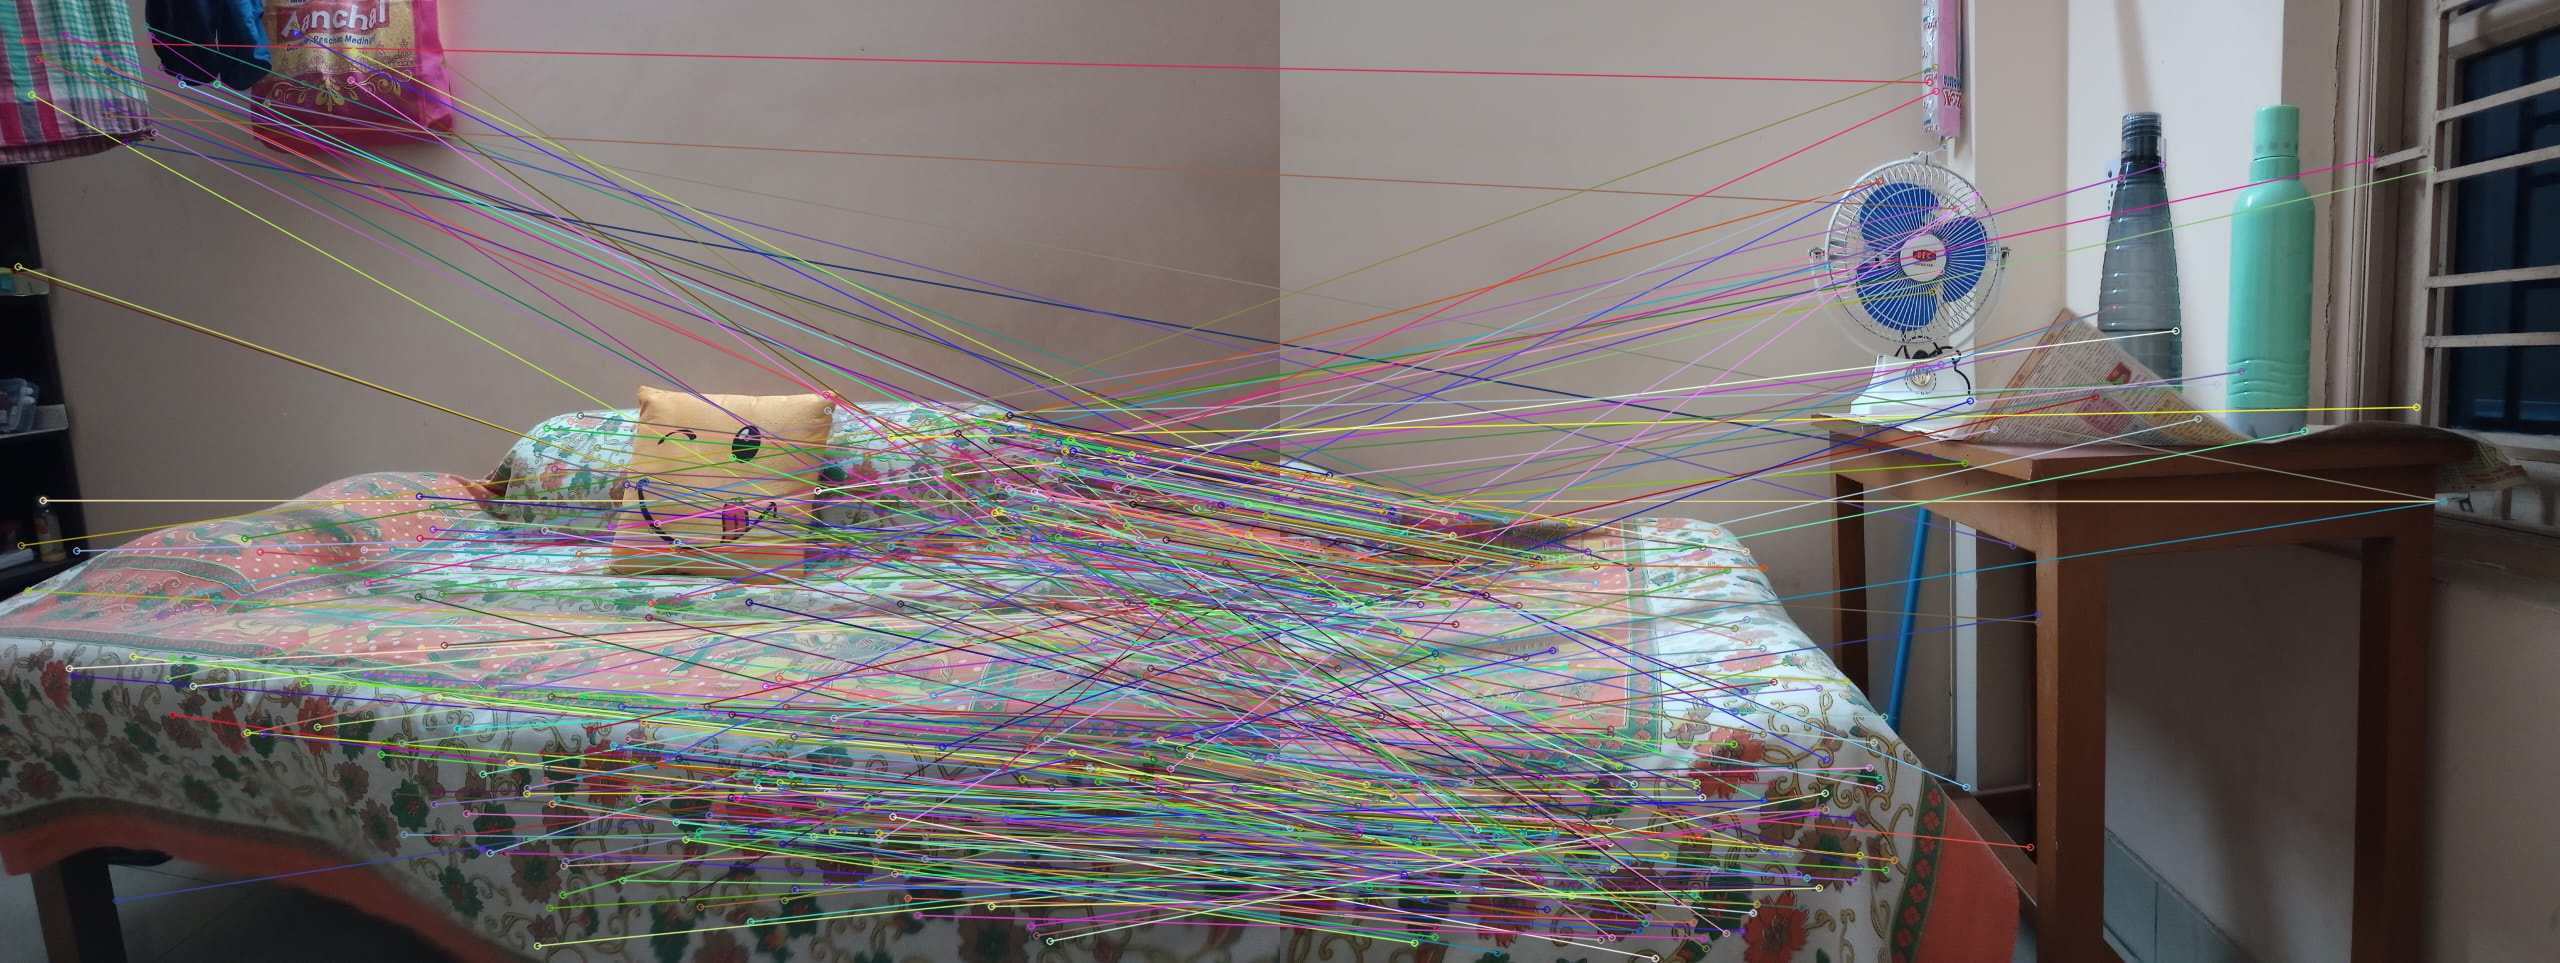
\includegraphics[width=0.8\textwidth]{matching2.jpg}
    \caption{Feature Matches between Images}
    \label{fig:matches}
\end{figure}
The results demonstrate improved stitching quality due to:
\begin{itemize}
    \item Enhanced feature detection from SIFT.
    \item Robustness through RANSAC.
    \item Smoothing at boundaries via custom blending masks.
\end{itemize}

Both image pairs (`left.jpg` + `right.jpg` and `left2.jpg` + `right2.jpg`) were stitched successfully.

\section{Conclusion}
This project presents a reliable and visually appealing image stitching pipeline using SIFT-based matching and blending masks. The smoothing window helps reduce seams, producing better results than naive image joining techniques.

\section{Future Improvements}
\begin{itemize}
    \item Integrate exposure compensation for better brightness consistency.
    \item Use multi-resolution pyramids for true multi-band blending.
    \item Extend to support 360° panoramic views with cylindrical projection.
\end{itemize}

\end{document}
